\documentclass[12pt, titlepage]{article}

\usepackage{fullpage}
\usepackage[round]{natbib}
\usepackage{multirow}
\usepackage{booktabs}
\usepackage{tabularx}
\usepackage{graphicx}
\usepackage{float}
\usepackage{hyperref}
\hypersetup{
    colorlinks,
    citecolor=blue,
    filecolor=black,
    linkcolor=red,
    urlcolor=blue
}

\input{../../Comments}
%% Common Parts

\newcommand{\progname}{Software Engineering} % PUT YOUR PROGRAM NAME HERE
\newcommand{\authname}{Team \#2, Team Name
\\ Zihao Du 
\\ Matthew Miller
\\ Firas Elayan
\\ Abhiram Neelamraju
\\ Michael Kim} % AUTHOR NAMES                  

\usepackage{hyperref}
    \hypersetup{colorlinks=true, linkcolor=blue, citecolor=blue, filecolor=blue,
                urlcolor=blue, unicode=false}
    \urlstyle{same}
                                


\newcounter{acnum}
\newcommand{\actheacnum}{AC\theacnum}
\newcommand{\acref}[1]{AC\ref{#1}}

\newcounter{ucnum}
\newcommand{\uctheucnum}{UC\theucnum}
\newcommand{\uref}[1]{UC\ref{#1}}

\newcounter{mnum}
\newcommand{\mthemnum}{M\themnum}
\newcommand{\mref}[1]{M\ref{#1}}

\begin{document}

\title{Module Guide for \progname{}} 
\author{\authname}
\date{\today}

\maketitle

\pagenumbering{roman}

\section{Revision History}

\begin{tabularx}{\textwidth}{p{3cm}p{2cm}X}
\toprule {\bf Date} & {\bf Version} & {\bf Notes}\\
\midrule
Jan 11 & 1.0 & Add Section Timeline and Reflection\\
Jan 15 & 1.0 & Revision 0\\
Apr 4 & 1.1 & Revision 1: Change some names of modules due to design change\\
Apr 4 & 1.1 & Revision 1: Update most of modules' type to Abstract Object since they are scenes in Unity and behave like singletons\\
Apr 4 & 1.1 & Revision 1: Updated traceability matrix and uses hierarchy\\
\bottomrule
\end{tabularx}

\newpage

\section{Reference Material}

This section records information for easy reference.

\subsection{Abbreviations and Acronyms}

\renewcommand{\arraystretch}{1.2}
\begin{tabular}{l l} 
  \toprule		
  \textbf{symbol} & \textbf{description}\\
  \midrule 
  AC & Anticipated Change\\
  AR & Augmented Reality\\
  \progname & AR social media application for McMaster students \\
  CRUD & Create, Read, Update and Delete\\
  DAG & Directed Acyclic Graph \\
  M & Module \\
  MG & Module Guide \\
  OS & Operating System \\
  R & Requirement\\
  SC & Scientific Computing \\
  SQL & Structured Query Language\\
  SRS & Software Requirements Specification\\
  UC & Unlikely Change \\
  UI & User Interface\\
  \bottomrule
\end{tabular}\\

\newpage

\tableofcontents

\listoftables

\listoffigures

\newpage

\pagenumbering{arabic}

\section{Introduction}

Decomposing a system into modules is a commonly accepted approach to developing
software.  A module is a work assignment for a programmer or programming
team~\citep{ParnasEtAl1984}.  We advocate a decomposition
based on the principle of information hiding~\citep{Parnas1972a}.  This
principle supports design for change, because the ``secrets'' that each module
hides represent likely future changes.  Design for change is valuable in SC,
where modifications are frequent, especially during initial development as the
solution space is explored.  

Our design follows the rules layed out by \citet{ParnasEtAl1984}, as follows:
\begin{itemize}
\item System details that are likely to change independently should be the
  secrets of separate modules.
\item Each data structure is implemented in only one module.
\item Any other program that requires information stored in a module's data
  structures must obtain it by calling access programs belonging to that module.
\end{itemize}

After completing the first stage of the design, the Software Requirements
Specification (SRS), the Module Guide (MG) is developed~\citep{ParnasEtAl1984}. The MG
specifies the modular structure of the system and is intended to allow both
designers and maintainers to easily identify the parts of the software.  The
potential readers of this document are as follows:

\begin{itemize}
\item New project members: This document can be a guide for a new project member
  to easily understand the overall structure and quickly find the
  relevant modules they are searching for.
\item Maintainers: The hierarchical structure of the module guide improves the
  maintainers' understanding when they need to make changes to the system. It is
  important for a maintainer to update the relevant sections of the document
  after changes have been made.
\item Designers: Once the module guide has been written, it can be used to
  check for consistency, feasibility, and flexibility. Designers can verify the
  system in various ways, such as consistency among modules, feasibility of the
  decomposition, and flexibility of the design.
\end{itemize}

The rest of the document is organized as follows. Section
\ref{SecChange} lists the anticipated and unlikely changes of the software
requirements. Section \ref{SecMH} summarizes the module decomposition that
was constructed according to the likely changes. Section \ref{SecConnection}
specifies the connections between the software requirements and the
modules. Section \ref{SecMD} gives a detailed description of the
modules. Section \ref{SecTM} includes two traceability matrices. One checks
the completeness of the design against the requirements provided in the SRS. The
other shows the relation between anticipated changes and the modules. Section
\ref{SecUse} describes the use relation between modules.

\section{Anticipated and Unlikely Changes} \label{SecChange}

This section lists possible changes to the system. According to the likeliness
of the change, the possible changes are classified into two
categories. Anticipated changes are listed in Section \ref{SecAchange}, and
unlikely changes are listed in Section \ref{SecUchange}.

\subsection{Anticipated Changes} \label{SecAchange}

Anticipated changes are the source of the information that is to be hidden
inside the modules. Ideally, changing one of the anticipated changes will only
require changing the one module that hides the associated decision. The approach
adapted here is called design for
change.

\begin{description}
\item[\refstepcounter{acnum} \actheacnum \label{acHardware}:] The specific
  hardware on which the software is running.
\item[\refstepcounter{acnum} \actheacnum \label{acPaginate}:] The algorithm for paginating
\item[\refstepcounter{acnum} \actheacnum \label{acFilter}:] The implementation of lecture/event filter
\item[\refstepcounter{acnum} \actheacnum \label{acProtocol}:] The protocol of server request and response
\item[\refstepcounter{acnum} \actheacnum \label{acServerData}:] The format of the server data packets
\item[\refstepcounter{acnum} \actheacnum \label{acListUI}:] The layout and styling of lecture/event list components UI
\item[\refstepcounter{acnum} \actheacnum \label{acDetailViewUI}:] The layout and styling of lecture/event detail view components UI
\item[\refstepcounter{acnum} \actheacnum \label{acMapInteract}:] Interaction with real-time map markers
\item[\refstepcounter{acnum} \actheacnum \label{acMapLayout}:] The look and feel of map layout
\item[\refstepcounter{acnum} \actheacnum \label{acUserUI}:] The layout and styling of User Profile component UI
\item[\refstepcounter{acnum} \actheacnum \label{acLoginUI}:] The layout and styling of User Login component UI
\item[\refstepcounter{acnum} \actheacnum \label{acFriendUI}:] The layout and styling of friend-related components UI
\item[\refstepcounter{acnum} \actheacnum \label{acARUI}:] The look and feel of AR Interface elements
\end{description}

\subsection{Unlikely Changes} \label{SecUchange}

The module design should be as general as possible. However, a general system is
more complex. Sometimes this complexity is not necessary. Fixing some design
decisions at the system architecture stage can simplify the software design. If
these decision should later need to be changed, then many parts of the design
will potentially need to be modified. Hence, it is not intended that these
decisions will be changed.

\begin{description}
\item[\refstepcounter{ucnum} \uctheucnum \label{ucInput}:]User input for in-app control
\item[\refstepcounter{ucnum} \uctheucnum \label{ucOS}:]OS on which the application is running
\item[\refstepcounter{ucnum} \uctheucnum \label{ucAccount}:]The information needed to create an account
\item[\refstepcounter{ucnum} \uctheucnum \label{ucDB}:]The Firebase real-time database implementation
\item[\refstepcounter{ucnum} \uctheucnum \label{ucBackend}:]The ASP.NET server implementation for real-time chatting and location sharing
\item[\refstepcounter{ucnum} \uctheucnum \label{ucAR}:]The Vuforia AR Camera implementation
\item[\refstepcounter{ucnum} \uctheucnum \label{ucAccess}:]The three access levels of users
\item[\refstepcounter{ucnum} \uctheucnum \label{ucUnity}:]The application will be implemented with Unity Engine
\end{description}

\section{Module Hierarchy} \label{SecMH}

This section provides an overview of the module design. Modules are summarized
in a hierarchy decomposed by secrets in Table \ref{TblMH}. The modules listed
below, which are leaves in the hierarchy tree, are the modules that will
actually be implemented.

\begin{description}
  \item [\refstepcounter{mnum} \mthemnum (\mref{mHH}):] Hardware-Hiding Module
  \item [\refstepcounter{mnum} \mthemnum (\mref{mDB}):] Database Module
  \item [\refstepcounter{mnum} \mthemnum (\mref{mServer}):] Server Module
  \item [\refstepcounter{mnum} \mthemnum (\mref{mAuth}):] Authentication Module
  \item [\refstepcounter{mnum} \mthemnum (\mref{mARCamera}):] AR Camera Module
  \item [\refstepcounter{mnum} \mthemnum (\mref{mARInterface}):] AR Interface Module
  \item [\refstepcounter{mnum} \mthemnum (\mref{mMap}):] Mapbox Module
  \item [\refstepcounter{mnum} \mthemnum (\mref{mRealTimeMap}):] RealTimeMap Module
  \item [\refstepcounter{mnum} \mthemnum (\mref{mUser}):] User Module
  \item [\refstepcounter{mnum} \mthemnum (\mref{mLec}):] Lecture Module
  \item [\refstepcounter{mnum} \mthemnum (\mref{mEvent}):] Event Module
  \item [\refstepcounter{mnum} \mthemnum (\mref{mDBConnector}):] DBConnector Module
  \item [\refstepcounter{mnum} \mthemnum (\mref{mAuthConnector}):] AuthConnector Module
  \item [\refstepcounter{mnum} \mthemnum (\mref{mUP}):] User Profile Module
  \item [\refstepcounter{mnum} \mthemnum (\mref{mUL}):] User Login Module
  \item [\refstepcounter{mnum} \mthemnum (\mref{mFM}):] Friend Manager Module
  \item [\refstepcounter{mnum} \mthemnum (\mref{mFR}):] Friend Request Module
  \item [\refstepcounter{mnum} \mthemnum (\mref{mFC}):] Friend Chat Module
  \item [\refstepcounter{mnum} \mthemnum (\mref{mADV}):] Activity Detail View Module
  \item [\refstepcounter{mnum} \mthemnum (\mref{mLDV}):] Lecture Detail View Module
  \item [\refstepcounter{mnum} \mthemnum (\mref{mEDV}):] Event Detail View Module
  \item [\refstepcounter{mnum} \mthemnum (\mref{mPF}):] Pagination and Filter Module
  \item [\refstepcounter{mnum} \mthemnum (\mref{mLL}):] Lecture List Manager Module
  \item [\refstepcounter{mnum} \mthemnum (\mref{mEL}):] Event List Manager Module
  \item [\refstepcounter{mnum} \mthemnum (\mref{mNoti}):] Notification Module
  \end{description}
  
  
  \begin{table}[H]
  \centering
  \begin{tabular}{p{0.3\textwidth} p{0.6\textwidth}}
  \toprule
  \textbf{Level 1} & \textbf{Level 2}\\
  \midrule
  
  {Hardware-Hiding Module} & ~ \\
  \midrule
  
  \multirow{7}{0.3\textwidth}{Behaviour-Hiding Module}
  & AR Interface Module\\
  & Real-time Map Module\\
  & User Module\\
  & Lecture Module\\
  & Event Module\\
  & User Profile Module\\
  & User Login Module\\
  & Friend Manager Module\\ 
  & Friend Request Module\\
  & Friend Chat Module\\
  & Lecture Detail View Module\\
  & Event Detail View Module\\
  & Lecture List Manager Module\\
  & Event List Manager Module\\
  & DBConnector Module\\
  & AuthConnector Module\\
  & Notification Module\\
  \midrule
  
  \multirow{3}{0.3\textwidth}{Software Decision Module}
  & Database Module\\
  & Server Module\\
  & Authentication Module\\
  & AR Camera Module\\
  & Mapbox Module\\
  & Activity Detail View Module\\
  & Pagination and Filter Module\\
  \bottomrule
  
  \end{tabular}
  \caption{Module Hierarchy}
  \label{TblMH}
  \end{table}
  
  \section{Connection Between Requirements and Design} \label{SecConnection}
  
  The design of the system is intended to satisfy the requirements developed in
  the SRS. In this stage, the system is decomposed into modules. The connection
  between requirements and modules is listed in Table~\ref{TblFRT}, \ref{TblNFRT}, \ref{TblNFRT-CONT}.
  
  \section{Module Decomposition} \label{SecMD}
  
  Modules are decomposed according to the principle of ``information hiding''
  proposed by \citet{ParnasEtAl1984}. The \emph{Secrets} field in a module
  decomposition is a brief statement of the design decision hidden by the
  module. The \emph{Services} field specifies \emph{what} the module will do
  without documenting \emph{how} to do it. For each module, a suggestion for the
  implementing software is given under the \emph{Implemented By} title. If the
  entry is \emph{OS}, this means that the module is provided by the operating
  system or by standard programming language libraries.  \emph{\progname{}} means the
  module will be implemented by the \progname{} software.
  
  Only the leaf modules in the hierarchy have to be implemented. If a dash
  (\emph{--}) is shown, this means that the module is not a leaf and will not have
  to be implemented.
  
  \subsection{Hardware Hiding Modules (\label{mHH})}
  
  \begin{description}
  \item[Secrets:]The data structure and algorithm used to implement the virtual
    hardware.
  \item[Services:]Serves as a virtual hardware used by the rest of the
    system. This module provides the interface between the hardware and the
    software. So, the system can use it to display outputs or to accept inputs.
  \item[Implemented By:] OS
  \end{description}
  
  \subsection{Behaviour-Hiding Module}
  \subsubsection{AR Interface Module (\label{mARInterface})}
  \begin{description}
  \item[Secrets:]How AR User Interface elements are created and displayed.
  \item[Services:]Creates 3D AR elements when notified by the AR Camera of a new valid target. Handles user input relating to AR UI elements.
  \item[Implemented By:] CampusConnections
  \item[Type of Module:] Abstract Object
  \end{description}
  
  \subsubsection{Real-time Map Module (\label{mRealTimeMap})}
  \begin{description}
  \item[Secrets:]How users, events and buildings are organized and displayed on the virtual map provided by the MapBox Module.
  \item[Services:]Displays points of interest such as buildings or events. Handles user interaction with points of interest. Displays user's avatar at their current location. Displays nearby friend locations on the map.
  \item[Implemented By:] CampusConnections
  \item[Type of Module:] Abstract Object
  \end{description}
  
  \subsubsection{User Module (\label{mUser})}
  \begin{description}
    \item[Secrets:]Data structure of a User.
    \item[Services:]Provides functionalities to interact with user data for other modules to use.
    \item[Implemented By:] CampusConnections
    \item[Type of Module:] Abstract Data Type
  \end{description}
  
  \subsubsection{Lecture Module (\label{mLec})}
  \begin{description}
    \item[Secrets:]Data structure of a Lecture.
    \item[Services:]Provides CRUD operations for users and administrators to interact with lecture data.
    \item[Implemented By:] CampusConnections
    \item[Type of Module:] Abstract Data Type
  \end{description}
  
  \subsubsection{Event Module (\label{mEvent})}
  \begin{description}
    \item[Secrets:]Data structure of an Event.
    \item[Services:]Provides CRUD operations for users and administrators to interact with event data.
    \item[Implemented By:] CampusConnections
    \item[Type of Module:] Abstract Data Type
  \end{description}
  
  \subsubsection{DBConnector Module (\label{mDBConnector})}
  \begin{description}
    \item[Secrets:]How users get access to the database data.
    \item[Services:]Provides database root for users to connect to.
    \item[Implemented By:] CampusConnections
    \item[Type of Module:] Abstract Object
  \end{description}
  
  \subsubsection{AuthConnector Module (\label{mAuthConnector})}
  \begin{description}
    \item[Secrets:]How current users get access to authentication information.
    \item[Services:]Provides current user information (e.g. if the email is verified) from authentication system for users
    \item[Implemented By:] CampusConnections
    \item[Type of Module:] Abstract Object
  \end{description}
  
  \subsubsection{User Profile Module (\label{mUP})}
  \begin{description}
    \item[Secrets:]How to display user profile and edit profile handlers
    \item[Services:]Allows users to view and edit (only for themselves) a user's profile.
    \item[Implemented By:] CampusConnections
    \item[Type of Module:] Abstract Object
  \end{description}
  
  \subsubsection{User Login Module (\label{mUL})}
  \begin{description}
    \item[Secrets:]The layout of account login/creation handlers and input fields
    \item[Services:]Allows users to enter account information to login to the system or create an account. Provide functionality to reset password as well.
    \item[Implemented By:] CampusConnections
    \item[Type of Module:] Abstract Object
  \end{description}
  
  \subsubsection{Friend Manager Module (\label{mFM})}
  \begin{description}
  \item[Secrets:]How to display friends as a list with corresponding handlers including adding, deleting, messaging and viewing.
  \item[Services:]Displays friends and as as a list and handle user input to add, message, delete a friend.
  \item[Implemented By:] CampusConnections
  \item[Type of Module:] Abstract Object
  \end{description}
  
  \subsubsection{Friend Request Module (\label{mFR})}
  \begin{description}
  \item[Secrets:]How to display friend requests as a list with corresponding handlers to accept or ignore requests.
  \item[Services:]Displays friend requests and as as a list and handle user input to accept or ignore a request.
  \item[Implemented By:] CampusConnections
  \item[Type of Module:] Abstract Object
  \end{description}
  
  \subsubsection{Friend Chat Module (\label{mFC})}
  \begin{description}
  \item[Secrets:]Procedures related to how chat messages are sent, received and handled on the client side.
  \item[Services:]Provides a link between the user interface and the backend server to allow users to chat in real time. Converts user input in the form of messages to data packets that are sent to the backend server.
  \item[Implemented By:] CampusConnections
  \item[Type of Module:] Abstract Object
  \end{description}
  
  \subsubsection{Event Detail View Module (\label{mEDV})}
  \begin{description}
  \item[Secrets:]How to inherit (\mref{mADV}) with activity type Event.
  \item[Services:]All services inherited from (\mref{mADV}) with activity type Event
  \item[Implemented By:] CampusConnections
  \item[Type of Module:] Abstract Object
  \end{description}
  
  \subsubsection{Lecture Detail View Module (\label{mLDV})}
  \begin{description}
  \item[Secrets:]How to inherit (\label{mADV}) with activity type lecture.
  \item[Services:]All services inherited from (\mref{mADV}) with activity type Event
  \item[Implemented By:] CampusConnections
  \item[Type of Module:] Abstract Object
  \end{description}
  
  \subsubsection{Lecture List Manager Module (\label{mLL})}
  \begin{description}
  \item[Secrets:]Implementation details of how lectures are displayed as a list with services inherited from (\mref{mPF}).
  \item[Services:]Displays a sequence of lectures as a list with pagination and filtering functionalities inherited from (\mref{mPF}).
  \item[Implemented By:] CampusConnections
  \item[Type of Module:] Abstract Object
  \end{description}
  
  \subsubsection{Event List Manager Module (\label{mEL})}
  \begin{description}
  \item[Secrets:]Implementation details of how events are displayed as a list with services inherited from (\mref{mPF}).
  \item[Services:]Displays a sequence of events as a list with pagination and filtering functionalities inherited from (\mref{mPF}).
  \item[Implemented By:] CampusConnections
  \item[Type of Module:] Abstract Object
  \end{description}
  
  \subsubsection{Notification Module (\label{mNoti})}
  \begin{description}
  \item[Secrets:] How users get a notification.
  \item[Services:]Displays a pop up window showing corresponding notification messages.
  \item[Implemented By:] CampusConnections
  \item[Type of Module:] Abstract Object
  \end{description}
  
  \subsection{Software Decision Module}
  \subsubsection{Database Module (\label{mDB})}
  \begin{description}
  \item[Secrets:]Database settings including structures of stored data, connection settings.
  \item[Services:]Provides CURD operations to database tables.
  \item[Implemented By:] Firebase
  \item[Type of Module:] Library
  \end{description}
  
  \subsubsection{Server Module (\label{mServer})}
  \begin{description}
  \item[Secrets:]How real-time data is sent to and received from clients.
  \item[Services:]Provides real-time communication endpoints for chatting and location sharing.
  \item[Implemented By:] Microsoft
  \item[Type of Module:] Library
  \end{description}
  
  \subsubsection{Authentication Module (\label{mAuth})}
  \begin{description}
  \item[Secrets:]Authentication token and user data related to authentication
  \item[Services:]Provides authentication token to existing users and prevent unauthorized users from accessing any accounts.
  \item[Implemented By:] Firebase
  \item[Type of Module:] Library
  \end{description}
  
  \subsubsection{AR Camera Module (\label{mARCamera})}
  \begin{description}
  \item[Secrets:]How AR targets are recognized.
  \item[Services:]Detects valid AR targets in the device's camera view and notifies the AR Interface module of the newly detected target.
  \item[Implemented By:] Vuforia
  \item[Type of Module:] Library
  \end{description}
  
  \subsubsection{Mapbox Module (\label{mMap})}
  \begin{description}
  \item[Secrets:]How to build and display customizable maps.
  \item[Services:]Provides different styles of interactive and customizable maps with basic functionalities (e.g. pan, center).
  \item[Implemented By:] Mapbox
  \item[Type of Module:] Library
  \end{description}
  
  \subsubsection{Activity Detail View Module (\label{mADV})}
  \begin{description}
    \item[Secrets:]How details of activities are displayed and changed.
    \item[Services:]Provides functionality for users and administrators to view, bookmakr, unbookmark; edit, and delete activities respectively.
    \item[Implemented By:] CampusConnections
    \item[Type of Module:] Generic Module
  \end{description}
  
  \subsubsection{Pagination and Filter Module (\label{mPF})}
  \begin{description}
    \item[Secrets:]Algorithm used for paginating and filter activities.
    \item[Services:]Displays activities as a paginated list which can be filtered by certain keyword.
    \item[Implemented By:] CampusConnections
    \item[Type of Module:] Generic Module
  \end{description}

\section{Traceability Matrix} \label{SecTM}

This section shows two traceability matrices: between the modules and the
requirements and between the modules and the anticipated changes.

% the table should use mref, the requirements should be named, use something
% like fref
\begin{table}[H]
\centering
\begin{tabular}{p{0.2\textwidth} p{0.6\textwidth}}
\toprule
\textbf{Req.} & \textbf{Modules}\\
\midrule
FR1-1 & \mref{mUL}\\
FR2-1 & \mref{mAuthConnector}, \mref{mDBConnector}, \mref{mUL}, \mref{mNoti}\\
FR2-2 & \mref{mAuthConnector}, \mref{mUP}, \mref{mDBConnector}, \mref{mNoti}\\
FR2-3 & \mref{mAuthConnector}, \mref{mUL}, \mref{mNoti}\\
FR2-4 & \mref{mAuthConnector}, \mref{mUL}, \mref{mNoti}\\
FR2-5 & \mref{mAuthConnector}, \mref{mUP}\\
FR2-6 & \mref{mUser}, \mref{mUP}, \mref{mDBConnector}, \mref{mNoti}\\
FR2-7 & \mref{mAuthConnector}, \mref{mUP}\\
FR2-8 & \mref{mUser}, \mref{mUP}, \mref{mDBConnector}\\
FR3-1 & \mref{mFM}, \mref{mDBConnector}, \mref{mNoti}\\
FR3-2 & \mref{mFM}, \mref{mDBConnector}, \mref{mNoti}\\
FR3-3 & \mref{mFC}, \mref{mServer}\\
FR3-4 & \mref{mFC}, \mref{mServer}\\
FR3-5 & \mref{mFC}, \mref{mServer}\\
FR3-6 & \mref{mFR}, \mref{mDBConnector}\\
FR4-1 & \mref{mUP}, \mref{mDB}, \mref{mEvent}, \mref{mEDV}, \mref{mADV}\\
FR4-2 & \mref{mUP}, \mref{mDB}, \mref{mLec}, \mref{mLDV}, \mref{mADV}\\
FR4-3 & \mref{mEvent}, \mref{mEDV}, \mref{mADV}, \mref{mDBConnector}, \mref{mAuthConnector}\\
FR4-4 & \mref{mLec}, \mref{mLDV}, \mref{mADV}, \mref{mDBConnector}, \mref{mAuthConnector}\\
FR4-5 & \mref{mEvent}\\
FR4-6 & \mref{mLec}\\
FR4-7 & \mref{mEvent}, \mref{mEL}, \mref{mPF}\\
FR4-8 & \mref{mLec}, \mref{mLL}, \mref{mPF}\\
FR5-1 & \mref{mARCamera}\\
FR5-2 & \mref{mARInterface}, \mref{mEvent}, \mref{mLec}\\
FR6-1 & \mref{mMap}, \mref{mRealTimeMap}, \mref{mServer}\\
\bottomrule
\end{tabular}
\caption{Trace Between Functional Requirements and Modules}
\label{TblFRT}
\end{table}

\begin{table}[H]
\centering
\begin{tabular}{p{0.2\textwidth} p{0.6\textwidth}}
\toprule
\textbf{Req.} & \textbf{Modules}\\
\midrule
LF-A1 & \mref{mARInterface} \mref{mFM}, \mref{mUP}, \mref{mLDV}, \mref{mEDV}, \mref{mLL}, \mref{mEL}, \mref{mUL}, \mref{mRealTimeMap}, \mref{mNoti}\\
LF-A2 & \mref{mARInterface} \mref{mFM}, \mref{mUP}, \mref{mLDV}, \mref{mEDV}, \mref{mLL}, \mref{mEL}, \mref{mUL}, \mref{mRealTimeMap}, \mref{mNoti}\\
LF-S1 & \mref{mARInterface} \mref{mFM}, \mref{mUP}, \mref{mLDV}, \mref{mEDV}, \mref{mLL}, \mref{mEL}, \mref{mUL}, \mref{mRealTimeMap}, \mref{mNoti}\\
LF-S2 & \mref{mARInterface} \mref{mFM}, \mref{mUP}, \mref{mLDV}, \mref{mEDV}, \mref{mLL}, \mref{mEL}, \mref{mUL}, \mref{mRealTimeMap}, \mref{mNoti}\\
UH-EOU1 & \mref{mARInterface} \mref{mFM}, \mref{mUP}, \mref{mLDV}, \mref{mEDV}, \mref{mLL}, \mref{mEL}, \mref{mUL}, \mref{mRealTimeMap}, \mref{mNoti}\\
UH-L1 & NA since it is a learning requirement related to document only\\
UH-UP1 & \mref{mARInterface} \mref{mFM}, \mref{mUP}, \mref{mLDV}, \mref{mEDV}, \mref{mLL}, \mref{mEL}, \mref{mUL}, \mref{mRealTimeMap}, \mref{mNoti}\\
UH-A1 & \mref{mARInterface} \mref{mFM}, \mref{mUP}, \mref{mLDV}, \mref{mEDV}, \mref{mLL}, \mref{mEL}, \mref{mUL}, \mref{mRealTimeMap}, \mref{mNoti}\\
P-SL1 & \mref{mARCamera}, \mref{mARInterface}\\
P-SL2 & \mref{mServer}, \mref{mRealTimeMap}\\
% P-SC1 & \mref{mDBConnector}, \mref{mServer}\\
% P-SC2 & \mref{mServer}\\
% P-SC3 & \mref{mRealTimeMap}\\
% P-SC4 & \mref{mServer}, \mref{mRealTimeMap}\\
% P-SC5 & \mref{mAuth}, \mref{mUP}, \mref{mDB}\\
% P-SC6 & \mref{mAuth}, \mref{mDB}\\
P-PA1 & \mref{mARCamera}\\
P-RF1 & \mref{mNoti}\\
P-RF2 & \mref{mDBConnector}, \mref{mServer}, \mref{mAuthConnector}\\
P-RF3 & \mref{mServer}\\
P-RF4 & \mref{mARInterface}, \mref{mNoti}\\
P-SE1 & \mref{mServer}\\
P-SE2 & \mref{mDB}, \mref{mAuth}\\
P-SE3 & \mref{mARInterface}\\
P-L1 & All modules (requirement related to coding style)\\
P-L2 & All modules (requirement related to coding style)\\
OE-EPE1 & NA since it is a device related requirement\\
OE-P1 & NA since it is a productization requirement\\
\bottomrule
\end{tabular}
\caption{Trace Between Non-Functional Requirements and Modules}
\label{TblNFRT}
\end{table}

\begin{table}[H]
\centering
\begin{tabular}{p{0.2\textwidth} p{0.6\textwidth}}
\toprule
\textbf{Req.} & \textbf{Modules}\\
\midrule
MS-M1 & NA since it is a requirement for maintainers\\
MS-S1 & NA since it is a requirement for maintainers\\
MS-A1 & NA since it is a device related requirement\\
S-A1 & \mref{mDB}, \mref{mAuth}, \mref{mUser}\\
S-A2 & \mref{mDB}, \mref{mAuth}, \mref{mUser}\\
S-A3 & \mref{mDB}, \mref{mAuth}, \mref{mUser}\\
S-A4 & \mref{mUL}, \mref{mNoti}\\
S-P1 & \mref{mDB}\\
S-P2 & \mref{mDB}, \mref{mAuth}\\
S-P3 & \mref{mRealTimeMap}\\
S-P4 & \mref{mServer}\\
S-P5 & \mref{mRealTimeMap}\\
S-US1 & \mref{mRealTimeMap}, \mref{mNoti}\\
CUL-C1 & \mref{mARInterface}, \mref{mRealTimeMap}, \mref{mUP}, \mref{mUL}, \mref{mFM}, \mref{mLDV}, \mref{mEDV}, \mref{mLL}, \mref{mEL}, \mref{mNoti}\\
COM-L1 & \mref{mDB}, \mref{mUser}, \mref{mEvent}, \mref{mLec}\\
COM-SC1 & \mref{mDB}, \mref{mUser}, \mref{mEvent}, \mref{mLec}\\
\bottomrule
\end{tabular}
\caption{Trace Between Non-Functional Requirements and Modules Cont.}
\label{TblNFRT-CONT}
\end{table}

\begin{table}[H]
\centering
\begin{tabular}{p{0.2\textwidth} p{0.6\textwidth}}
\toprule
\textbf{AC} & \textbf{Modules}\\
\midrule
\acref{acHardware} & \mref{mHH}\\
\acref{acPaginate} & \mref{mPF}\\
\acref{acFilter} & \mref{mPF}\\
\acref{acProtocol} & \mref{mServer}\\
\acref{acServerData} & \mref{mServer}\\
\acref{acListUI} & \mref{mLL}, \mref{mEL}\\
\acref{acDetailViewUI} & \mref{mADV}, \mref{mLDV}, \mref{mEDV}\\
\acref{acMapInteract} & \mref{mRealTimeMap}, \mref{mMap}\\
\acref{acMapLayout} & \mref{mRealTimeMap}\\
\acref{acUserUI} & \mref{mUP}\\
\acref{acLoginUI} & \mref{mUL}\\
\acref{acFriendUI} & \mref{mFM}, \mref{mFR}, \mref{mFC}\\
\acref{acARUI} & \mref{mARInterface}\\
\bottomrule
\end{tabular}
\caption{Trace Between Anticipated Changes and Modules}
\label{TblACT}
\end{table}

\section{Use Hierarchy Between Modules} \label{SecUse}

In this section, the uses hierarchy between modules is
provided. \citet{Parnas1978} said of two programs A and B that A {\em uses} B if
correct execution of B may be necessary for A to complete the task described in
its specification. That is, A {\em uses} B if there exist situations in which
the correct functioning of A depends upon the availability of a correct
implementation of B.  Figure \ref{FigUH} illustrates the use relation between
the modules. It can be seen that the graph is a directed acyclic graph
(DAG). Each level of the hierarchy offers a testable and usable subset of the
system, and modules in the higher level of the hierarchy are essentially simpler
because they use modules from the lower levels.

\begin{figure}[H]
\centering
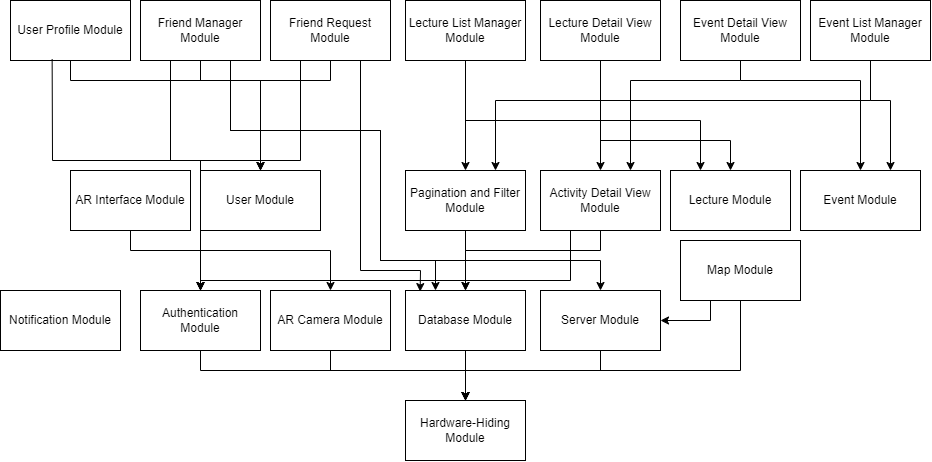
\includegraphics[width=0.9\textwidth]{UsesHierarchy.png}
\caption{Use hierarchy among modules}
\label{FigUH}
\end{figure}

\section{User Interfaces}

User interfaces can be found \href{https://www.figma.com/file/4kCzs4a1iqRLSKAwUbJREh/UI-Feedback?type=design&node-id=0%3A1&mode=design&t=6hfaqfbeFLTKRl9E-1}{here}.

\section{Timeline}
\begin{table}[H]
\centering
\begin{tabular}{p{0.35\textwidth} p{0.3\textwidth}  p{0.3\textwidth}}
\toprule
Module Name & Team Member & Due Date \\
\midrule
User & Zihao Du & Nov 15, 2023\\
Account & Zihao Du & Dec 4, 2023\\
Database & Zihao Du & Dec 4, 2023\\
Friend Request & Zihao Du & Jan 10, 2024\\
Friend Manager & Zihao Du & Jan 15, 2024\\
Chat & Waseef Nayeem, Zihao Du & Jan 15, 2024\\
Mapbox & Waseef Nayeem & Jan 15, 2024\\
Server & Waseef Nayeem & Jan 15, 2024\\
Authentication & Michael Kim & Jan 15, 2024\\
Permission & Michael Kim & Jan 15, 2024\\
User Profile & Michael Kim & Jan 15, 2024\\
Lecture & Abhiram Neelamraju & Jan 15, 2024\\
Lecture List Manager & Abhiram Neelamraju & Jan 15, 2024\\
Pagination and Filter & Abhiram Neelamraju, Firas Elayan & Jan 15, 2024\\
Activity Detail View & Matthew Miller & Jan 17, 2024\\
Event Detail View & Matthew Miller & Jan 17, 2024\\
Lecture Detail View & Matthew Miller & Jan 17, 2024\\
Event & Firas Elayan & Jan 17, 2024\\
Event List Manager & Firas Elayan & Jan 17, 2024\\
User Login & Michael Kim & Jan 17, 2024\\
RealTimeMap & Waseef Nayeem & Jan 17, 2024\\
Mapbox Manual Test & Waseef Nayeem & Jan 26, 2024\\
Server Manual Test & Waseef Nayeem & Jan 26, 2024\\
\bottomrule
\end{tabular}
\caption{CampusConnections Module Completion Timeline}
\end{table}

\begin{table}[H]
\centering
\begin{tabular}{p{0.35\textwidth} p{0.3\textwidth}  p{0.3\textwidth}}
\toprule
Test Name & Team Member & Due Date \\
\midrule
Database Manual Test & Zihao Du & Jan 26, 2024\\
User Unit Test & Zihao Du & Jan 26, 2024\\
Authentication Manual Test & Michael Kim & Jan 26, 2024\\
Event Unit Test & Firas Elayan & Jan 26, 2024\\
Lecture Unit Test & Abhiram Neelamraju & Jan 26, 2024\\
Map Scene Manual Test & Waseef Nayeem & Feb 2, 2024\\
ARCamera &Waseef Nayeem, Zihao Du & Feb 2, 2024\\
ARCamera Manual Test &Waseef Nayeem, Zihao Du & Feb 2, 2024\\
ARInterface & Waseef Nayeem, Zihao Du & Feb 2, 2024\\
AR Scene Manual Test & Waseef Nayeem, Zihao Du & Feb 2, 2024\\
Friend Scene Manual Test & Zihao Du & Feb 2, 2024\\
User Login Scene Manual Test & Michael Kim & Feb 2, 2024\\
User Profile Scene Manual Test & Michael Kim & Feb 2, 2024\\
List View Manual Test & Abhiram Neelamraju, Firas Elayan & Feb 2, 2024\\
Detail View Manual Test & Matthew Miller & Feb 2, 2024\\
Integration Test for Rev 0 & All & Feb 5, 2024\\
\bottomrule
\end{tabular}
\caption{CampusConnections Test Timeline}
\end{table}
\newpage{}

\appendix

\section{Reflection}

The information in this section will be used to evaluate the team members on the
graduate attribute of Problem Analysis and Design.  Please answer the following questions:

\begin{enumerate}
  \item What are the limitations of your solution?  Put another way, given
  unlimited resources, what could you do to make the project better? (LO\_ProbSolutions)
  
	One of the main limitations of the solution is the time allotted for this project. This is an ambitious project that has various impressive features, but due to the time limitation, we have to limit the number of features and leave some good designs in the waiting room. One way to improve the project is to iterate over the project for several rounds when implementing and ranking all features by significance. For the very first round, we only import the fundamental features, and in the later round, we will work on other less important features and UI. Currently here is a list of features to implement in this round:
	\begin{itemize}
	\item Real-time system server
	\item Multi-user location-sharing map
	\item List view of events/lectures with pagination and filtering
	\item Detail View of events/lectures
	\item User Profile Page
	\item Friend Chatting System
	\end{itemize}
 And there are also some features already on the list for the next round
 like Event sharing, Heat map, etc.
 
 	Another limitation is the budget. Since we are using some third-party library (e.g. AR Engine) and the budget is limited, we can only use the free plan for now. The free plan has limited capacity and watermark, which affects the user experience and limits the features we can implement. To improve this, we need to limit the number of target buildings on the map and provide only a portion of indoor AR features for the first release.
 	
 	For this project, data-sharing restrictions limit the features as well. Since the administrator needs to feed the community up-to-date information about campus activities. If the administrator cannot provide good resources, the application is much less helpful for its user. One way to solve the problem is to invite club leaders or even McMaster staff as our administrators so that the community can be always active.
  \item Give a brief overview of other design solutions you considered.  What
  are the benefits and tradeoffs of those other designs compared with the chosen
  design?  From all the potential options, why did you select documented design?
  (LO\_Explores)
  
  We are implementing this application with Unity, using Firebase Database and Authentications. We also designed an ASP.NET server for multi-user chatting and location sharing.
  The benefit of using Unity Engine is it has great support for AR features. Our AR Engine, Vuforia works perfectly fine with Unity.  Also, we can make use of lots of 3D/2D object from Unity Asset Store when implementing maps and our interfaces, which provides an immersive user experience.  Unity also has a very active community and detailed documentation as well.  Compared to some other front-end frameworks like React, Unity doesn't have good support for UI components as a tradeoff. However, the team thinks map and AR components are much more important features than layout and UI.
  	We are also using Firebase Real-time database, a non-relational database for this project. Compared to relational databases like Microsoft SQL,  it is flexible and updates in almost real-time. As a product of Firebase, it collaborates with Firebase Authentication System very well. It provides protection rules for reading and writing on the database side which prevent users from bypassing the front end and attacking the database directly. As a tradeoff, the data in the database are not well organized by schemas like relational databases, and it may be quite difficult to extend and maintain in the future.
\end{enumerate}

\newpage
\bibliographystyle {plainnat}
\bibliography{../../../refs/References}

\newpage{}

\end{document}